This research is conducted as part of the final thesis of Mitchell Quinn Puls, Technical Computing student at the Amsterdam University of Applied Sciences. This research is about the effects of a high amount of computers, processing a vast amount of data. This research is in assignment from CERN in Switzerland. 
\section{CERN}
CERN is a European organization for  nuclear research, situated in Geneve Switserland. CERN was founded in 1954 and is one of Europe's first join ventures. The main goal is to study the fundamental structure of the universe, by researching matter and particles using purpose built particle accelerators and detectors. Particle accelerators beam particles to high energies, before colliding them against each other against or a stationary object. Detectors record and observe this collision. One of these detectors is ALICE
\section{ALICE}
ALICE stands for A Large Ion Collider Experiment, and is a detector mounted on the Large Hadron Collider at CERN.  ALICE's main function is to study matter at extreme energy densities, where matter turns into a form called quark-gluon plasma. Everything in the universe is made from protons, neutrons (except hydrogen which does not have any neutrons) and electrons. Protons and neutrons are then build up with quarks and bound together with something called a gluon. Quark-gluon plasma matter that appeared at the very start of the big bang, and is the thing that binds the gluons and quarks together. CERN wants to observe this matter. The way they achieve this, is by shooting two lead ions against each other. This produces a heat that is over 100,000 times hotter than the center of the Sun. This breaks the bounds between the quarks and the gluons and makes the quark-gluon plasma visible.
\subsection{Upgrade}
In July 2018 the accelerator will be stopped for around 18 months for a planned upgrade of the ALICE detector. (van der Lee, 2017, p. 1) During this period, CERN is upgrading it's hardware and software. This upgrade is in collaboration with various schools and universities throughout Europe, including the Amsterdam University of Applied Science. One of these upgrades is an algorithm for Load Balancing. In 2020, ALICE will restart with it's new upgraded detector. ("Technical Design Report for the Upgrade of the Online Offline Computing System", 2015, p. i)

\section{Load Balancing}
The data stream that comes from ALICE is equal to about 1.1 Terabyte per second. All of this data comes in what is known as a heartbeat. This heartbeat gets distributed over 268 First Level Processors and funneled through	1500 Event Processing Nodes. The efficient distribution of this process, and also the handling of data in case of a failure in the system, is what is known as Load Balancing. All of these computers would be monitored by an Information Node.

\section{Research}
This research is a continuation of a previous research done by Heiko van der Heijden. His results show that of the two algorithms tested, Re-initialization and Blacklist, that the Blacklist algorithm has fewer Time Frames lost.\\
Even though the same ratio of FLPs to EPNs that is situated at CERN was used (1/6), there were fewer computers used than at CERN. Because of this it is not sure whether or not the Information Node is able to handle 1700+ computers as compared to the 15 computers used in the experiment. This research is focused on the capability of the Information Node to monitor a higher number of FLPs and EPNs and what the effects are on the results compared to the previous experiment.

\section{Research Model}
Contrary to the previous research, which used a cluster of computers situated at Nikhef Amsterdam, this research will be conducted using a cluster of Raspberry Pi's. This decision has been made because of an unfortunate failure of communication from Nikhef about the availability of the cluster for this research period. The first step is to recreate the previous experiment which was focused around the various ticktimes of Zookeeper.
\newpage

~\\\textbf{The main purpose of this research is to both validate the results from the previous experiment, but also to validate the new Raspberry Pi cluster to confirm that this is a valid way to conduct this experiment. After recreating the first experiment, the same experiment will be conducted with a higher numbers of computers to see if this has an effect on the Information Node.} \\~\\
An overview can be seen in figure ~\ref{fig:ResearchModel}

\begin{figure}[htb]
	\centering
	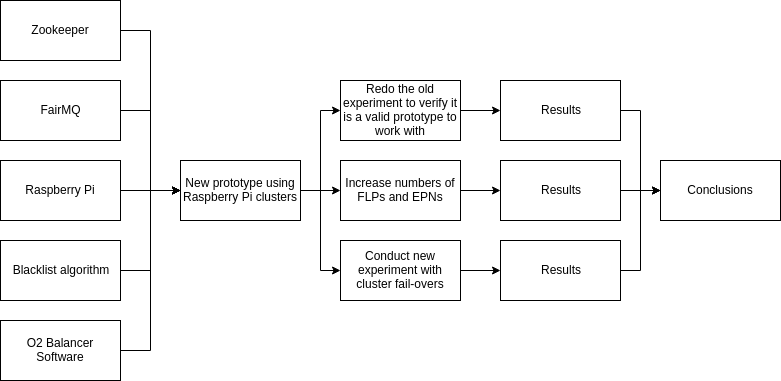
\includegraphics[scale=0.5]{./graphics/ResearchModel.png}
	\caption{Research model}
	\label{fig:ResearchModel}
\end{figure}

~\\ All technical documentation of what everything is will be explained in the next section including the definition of the experiments.
The next chapter will explore more in depth of the prototype made for the experiment and it's difficulties that came with it. The following chapter looks at the results from the  executed experiments. After this follows an analysis of the results of the experiment. Finally a conclusion and recommendations.